\chapter{Implementierung}
In diesem Kapitel wird zunächst die Implementierung der verschieden Ansätze in C++ behandelt. Hierbei wird auch auf die Besonderheiten des FPGA eingegangen. Des weiteren wird erläutert, wie der FPGA programmiert wird, vor allem in Hinblick auf die Parallelisierung der einzelnen Komponenten.
\section{Implementierung in C++}
Für die erste Implementierung der Voraussagefunktion wurde der Code von \cite{IMPL} aus Python in C++ übersetzt und an die Eigenschaften eines FPGA angepasst. In Abbildung 4.1 sind die Kernfunktionen des Programmcodes dargestellt. Die Funktion \textit{predict()} liefert die Berechnung der Formel $\dfrac{1}{1+\exp(-(\beta_0+x_i^T\beta))}$. Die Koeffizienten $\beta$ sind hier als Array $coefficients[\text{ }]$ gespeichert, zudem gibt es für die Batch-Realisierung ein Hilfsarray $tmp\textit{\_}coefficients[\text{ }]$. Der Datentyp \textit{DATA\_TYPE} kann hier zum einen Als Gleitkommazahl (\textit{float}), zu anderen als Fixkommazahl (\textit{ap\_fixed}) deklariert werden. Die Wahl für den Fixkomma-Datentyp fällt auf ein von Xilinx selbst bereitgestelltes Konstrukt \textit{ap\_fixed}, da es für das FPGA optimiert wurde und hier eine Vielzahl an Konfigurationen vorgenommen werden können. Die Gesamtanzahl der für eine Instanz belegten Bits wurde auf 16 festgelegt, davon ein Vorzeichenbit und 4 Vorkommastellen. Durch die Einstellung \textit{AP\_RND\_CONV} wird die Zahl, zum Beispiel nach einer Divisionsberechnung auf den nächsten repräsentierbaren Wert gerundet. Die Rundungsrichtung ist dabei abhängig von dem am wenigsten signifikanten Bit. Ist dieses gesetzt wird gegen $+\infty$, andernfalls gegen $-\infty$ gerundet.\cite{XIL2}
Um einem eventuellen Overflow der Zahl entgegenzuwirken wählt man die Einstellung \textit{AP\_SAT\_SYM}. Im Fall eines Positiven Overflows wird hierbei der höchste, bei einem negativen Overflow der kleinste darstellbare Wert gewählt.\cite{XIL2} Die FPGA Einstellung \textit{pragma HLS LOOP FLATTEN} sorgt für eine Parallelisierung der Schleife auf dem FPGA. Das funktioniert allerdings nur, wenn innerhalb der Schleife auf immer andere Ziele geschrieben wird.\\ In der Funktion \textit{predict()} zum Beispiel wird die Variable \textit{yhat} immer wieder neu gesetzt, sodass eine Paralleliserung hier nicht möglich ist. 
\begin{figure}[ht]
\centering
\begin{lstlisting}
/* Voraussage treffen anhand logistischer Regression */
DATA_TYPE predict(){
    DATA_TYPE yhat = coefficients[0];
	for(int i=0; i<FEATURE_COUNT; i++){
		yhat+=coefficients[i+1]*features[i];
	}
	float tmp_yhat=-yhat;
	DATA_TYPE predicted=1.0f/(1.0f+hls::expf(tmp_yhat));
	return predicted;
}
\end{lstlisting}
\begin{lstlisting}
void learn(){
    DATA_TYPE predicted=predict();
    DATA_TYPE error=label-predicted;
    tmp_coefficients[0]+=error;
	for(int i=0; i<FEATURE_COUNT; i++){
		#pragma HLS LOOP FLATTEN
		tmp_coefficients[i+1]+=error*features[i];
	}
	/* Batch Update der Koeffizienten */
	batch_count++;
	if(batch_count>=BATCH_SIZE){
		batch_count=0;
		coefficients[0]+=lrate*tmp_coefficients[0]/BATCH_SIZE;
		tmp_coefficients[0]=0;
		for(int i=1; i<FEATURE_COUNT+1; i++){
			#pragma HLS LOOP FLATTEN
			coefficients[i]=punish(i) + 
				lrate*tmp_coefficients[i]/BATCH_SIZE;
			tmp_coefficients[0]=0;
		}
	}
}
\end{lstlisting}
\caption{Codes des Perzeptrons}
\end{figure}
\\Die Funktion \textit{hls::expf()} wird von Xilinx geliefert und dient als Realisierung der Expotentialfunktion und ist für FPGAs optimiert.\\ 


Um die High-Performance Schnittstelle über PCIe von \cite{DILL} voll ausnutzen zu können wurde eine Trennung der Codeteile vorgenommen, damit ein Teil des Algorithmus auf dem FPGA und ein Teil auf dem Hostcomputer laufen kann. Der Hostrechner übernimmt hier die Vorbereitung der Daten und die Äußeren Schleifendurchläufe. Es werden immer die einzelnen Variablen mit dem dazugehörigen Label an den FPGA gesendet, welcher dann je nach Konfiguration damit trainiert oder eine Voraussage trifft. Der Vorteil hierbei ist, dass auf dem FPGA mehrere logistische Regressionen gleichzeitig implementiert sind, die mit verschiedenen Parametern (zum Beispiel einem C für die Fehlerbestrafungsgewichtung oder unterschiedlichen Lernraten) initialisiert wurden.\\
Die Methode \textit{punish()} wendet die ausgewählte Regularisierungsmethode auf das Batch Update an. Es wurden keine Regularisierung, L1- und L2-Regularisierung implementiert, sodass für den selben Trainingsdurchlauf verschiedene Methoden getestet werden können. in Abbildung 4.2 ist die Funktion als Programmcode dargestellt.\\
\begin{figure}[ht]
\centering
\begin{lstlisting}
/*Punishment sollte vorinitialisiert werden, da Konstant abhaengig von der Regularisierungsgewichtung, der Batchgroesse und der Lernrate */

DATA_TYPE punishment=lrate*c/BATCH_SIZE

void punish(int i){
	/*L1 Regularisierung*/
	if(method==1){
		return coefficients[i]-punishment*sign(coefficients[i]);
	}
	/*L2 Regularisierung*/
	if(method==2){
		return coefficients[i]*(1-punishment);
	}
	return coefficients[i];
	    
}
\end{lstlisting}
\caption{Implementierte Regularisierungsmethoden}
\end{figure}\\
Die angewendete L1- und L2-Regularisierung für das Koeffizientenupdate ergibt sich aus der Ableitung der Kostenfunktion, welche um den Regularisierungsterm erweitert wurde.
für LASSO ergibt sich der Term aus:
\begin{displaymath}
\beta_i^{(l+1)}=\beta_i^{(l)}+\eta^{(l)} \cdot \dfrac{\partial}{\partial \beta_i} \left( J(\beta)-\frac{C}{m} \cdot | \beta_i^{(l)} |\right)
\end{displaymath}
Mit $x_i \in \vec x_l$. Da die Betragsfunktion nicht differenzierbar ist behilft man sich mit der Vorzeichenfunktion \textit{sign()}. Es entsteht damit folgender Term für das Update \cite{L1C}:
\begin{displaymath}
\beta_i^{(l+1)} = \beta_i^{(l)} + \eta^{(l)} \cdot \frac{1}{m} \sum_{i=l\cdot m + 1}^{(l+1) \cdot m} (y_i-\pi(\vec x_i)) \cdot x_i -\eta^{(l)}\cdot \frac{C}{m} \cdot sign(\beta_i^{(l)})
\end{displaymath}
Für die Ridge Regression ist der Ableitungsterm deutlich einfacher zu bestimmen. Aus 
\begin{displaymath}
\beta_i^{(l+1)}=\beta_i^{(l)}+\eta^{(l)} \cdot \dfrac{\partial}{\partial \beta_i} \left( J(\beta)-\frac{C}{2m} \cdot \sum_{k=1}^d (\beta_k^{(l)})^2 \right)
\end{displaymath} wird \cite{HER2}
\begin{displaymath}
\beta_i^{(l+1)} = \beta_i^{(l)} \cdot \left(1-\eta^{(l)}\frac{C}{m}\right) + \eta^{(l)} \cdot \frac{1}{m} \sum_{i=l\cdot m + 1}^{(l+1) \cdot m} (y_i-\pi(\vec x_i)) \cdot x_i
\end{displaymath}\\
Um die Datenverteilung auf dem FPGA zu gewährleisten wurde sowohl eine Verteiler- als auch eine Sammlerklasse implementiert. Diese sind für dafür zuständig den Datenstrom von Daten und Konfigurationsparametern auf die jeweiligen Perceptrons zu verteilen beziehungsweise von diesen einzusammeln. Die Sammlerklasse markiert zusätzlich noch die ausgegebenen Daten mit der Identifikation des jeweiligen Perceptrons, damit die Ergebnisse nach einem Durchlauf zugeordnet werden können.
Die Verteilerklasse übernimmt bei der Implementierung mit der 16-Bit Fixkommazahl zudem die Aufteilung des Eingangstroms, da über die 32-Bit Ausgangsleitung des Xillybus-Blocks jeweils zwei Datenpunkte pro Übertragung versendet werden können.
\section{Implementierung als Blockdesign}
Um Auf dem FPGA zu implementieren, muss der Code für den Verteiler, den Sammler und das Perceptron in eine IP (Intelectual Property) umgewandelt werden. Die IP-Blöcke werden für das Blockdesign wie in Abbildung 4.4 angeordnet und verbunden. Hierbei sind die Perceptrons für Daten aus der MNIST (Modified National Institute of Standards and Technology) Datenbank konfiguriert, das heißt jedes Perceptron hat einen Variablenspeicher von 784 Features (28x28 Pixel) und jeweils 785 Koeffizienten und Hilfskoeffizienten.\\
Die MNIST Datenbank ist eine Sammlung handgeschriebener Ziffern, komprimiert, zentriert und normalisiert auf 28x28 Pixel mit Werten zwischen 0-256, welche die Farben von Weiß nach Schwarz repräsentieren. Die 60.000 Trainingsvariablen wurden zu jeweils gleichen Teilen aus der NIST (National Institute of Standards and Technology) Testdatenbank und der NIST Trainingsdatenbank entnommen, gleiches gilt für die 10.000 Variablen große Testmenge. Diese Anpassung wurde vorgenommen, da die Variablen der Testmenge unter Mitarbeitern des Volkszählungsamts erhoben wurden und deutlich besser zu klassifizieren sind als die unter Studenten erhobenen Daten der Trainingsmenge. Die Daten der Trainingsmenge wurden von circa 250 Teilnehmern erhoben, von denen keine Einträge in der Testmenge eingefügt wurden \cite{MNIST}.\\
\begin{figure}[ht]
\centering
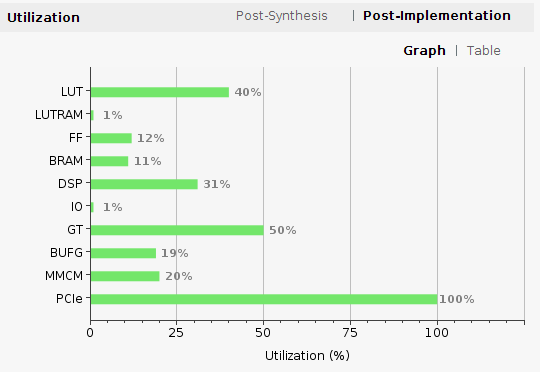
\includegraphics[scale=1.0]{bilder/auslastung1}
\caption{Auslastung auf dem FPGA mit 16-Bit Fixkommazahl und 8 Perceptrons}
\end{figure}\\
Die Auslastung des FPGA für diese Implementierung beträgt in etwa 50\% (siehe Abbildung 4.3), sodass auch 16 Perceptrons parallel geschaltet werden können. Für die bildliche Darstellung in dieser Arbeit wäre dies jedoch ein zu großes Diagramm. Für Datensätze mit mehr Features als MNIST erhöht sich zudem die Auslastung, da jedes Perceptron zwei Koeffizientenvektoren und einen Zwischenpuffer mit einer Länge gleich der Anzahl der Features im Speicher haben muss. Daher können für diese Datensätze keine 16 oder sogar weniger als 8 Perceptrons in das Design eingefügt werden.
%TEsten ob das funktioniert %

 \begin{figure}[ht]
\centering
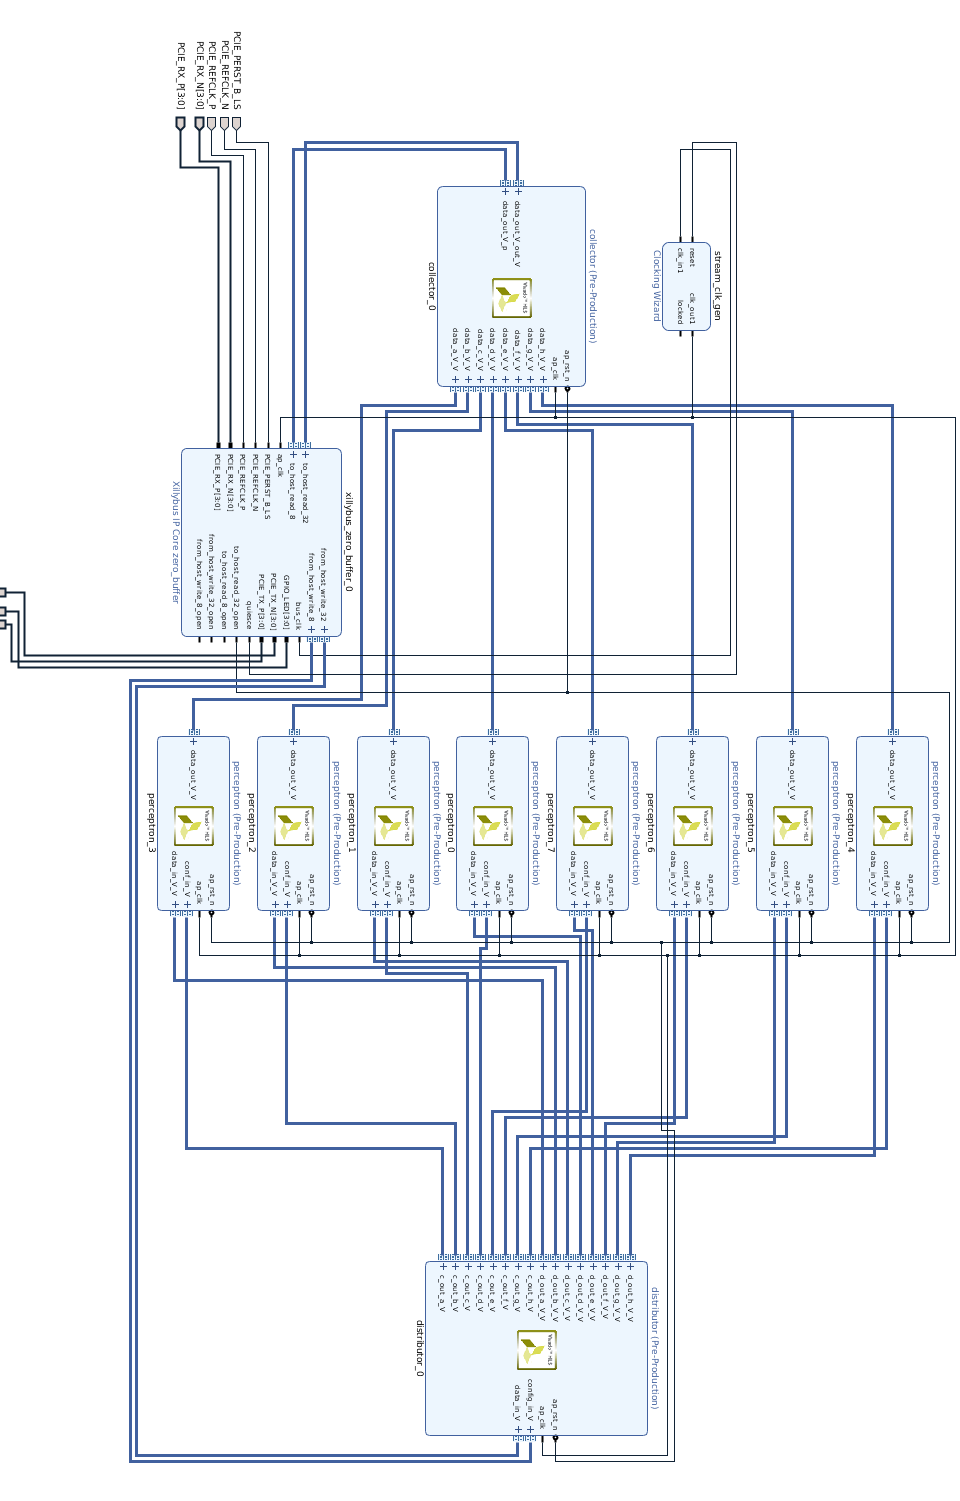
\includegraphics[scale=0.7]{bilder/blockdesign}
\caption{Das Blockdesign auf dem FPGA}
\end{figure}\\
